\documentclass[letterpaper,12pt]{texMemo}

\usepackage{graphicx}

\memoto{The School House Board of Managers}
\memofrom{The School House South Stack Exhaust Fan Committee}
\memosubject{Initial Timer Investigation}
\memodate{Monday, July 27, 2020}
% \memologo{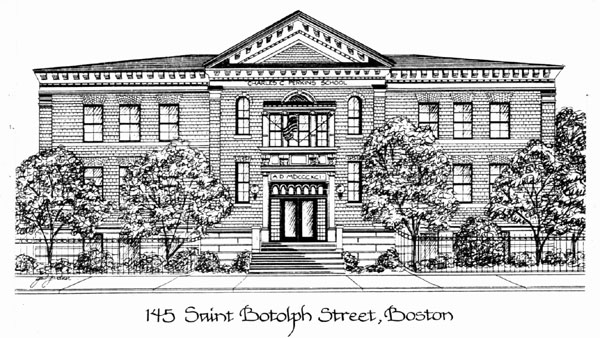
\includegraphics[height=8\baselineskip]{schoolhouse-etching.jpg}}
% \logo{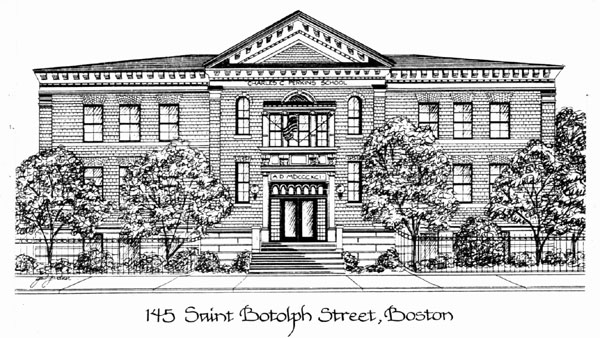
\includegraphics[width=0.3\textwidth]{schoolhouse-etching.jpg}}

% Add vertical space between paragraphs
\setlength{\parskip}{\baselineskip}

\begin{document}
\maketitle

\section{Abstract}

At the request of the President of the Board of Managers we have undertaken
management of the timer that controls the attic fan component of the South
stack kitchen and bathroom exhaust fans. Our initial investigation indicates
that the timer is not powered, and that the timer may be set incorrectly.

\section{Background}

On July 11, 2020, Dave Reed was alerted to food smells
in an apartment in the south corner of the building (corner of Saint
Botolph St and the School House parking lot). Dave was able to
determine that the smells were the result of cooking in the basement
apartment, and the exhaust fan in that apartment blowing the odors
into other units in the same exhaust fan stack. The exhaust was not
blown out of the building because the exhaust fan in the attic is on
a timer which is set to turn off at approximately 9:00 p.m.

Dave Reed subsequently contacted us to ask if we could manage the
exhaust fan timer set up. The timer was initially put in place because
the previous owners of apartment 34 were bothered by the noise of
the exhaust fan if it ran all night.

\section{Timer Introduction}

On July 23, 2020, Dave Reed met with the committee to explain
the timer. Dave showed us the timer in the electrical and water closet at
the far end of the storage room on the ground floor. The timer unit appears
to be wired to the electrical panel. The instructions for the timer unit are
on a sheet of paper stored inside the unit.

According to the instructions the unit is an Intermatic GM40AV Series
GRASSLIN General Purpose Electromechanical Commercial Time Switches unit.

\section{Initial Investigation}

We did an initial investigation of the timer unit on Sunday July 26, 2020.
That investigation has revealed two issues. The timer does not appear
to be receiving power and the timer does not appear to be set correctly.

\subsection{Timer is not powered}

The timer unit does not appear to be powered. There are two reasons
why we think this is the case:

\begin{enumerate}
\item The power light is not illuminated
\item The timer did not move or change in any way over the course of 11 hours
\end{enumerate}

The first time check was at 10:15 a.m. (see figures 1 and 2). We picked up the
instructions, studied the current settings, and took photos. At this time it
appeared that the unit was not receiving power. We took another photo
(see figure 3) at 2:30 p.m. and confirmed that the unit had not moved at
all in the 4 hour interval since the first photos. Two more photos were taken,
the first at 5:20 p.m. (figure 4) and the second at 9:20 p.m. (figure 5) and
both show that the timer has not moved at all. The status lights were both
dark in all photos.

\subsection{Timer is not set correctly}

The timer instructions say that when the trippers (white tabs, 4 per hour)
are OUT, the power is ON, and
when the trippers are IN, the power is OFF. At present the trippers are set
to OUT (power ON) from 8:15 p.m. to 9:00 a.m. The
trippers are set to IN (power OFF) from 9:00 a.m. to 8:15 p.m.
These settings seem to be the opposite of what is desired.

We cannot confirm this because the unit is not powered. Once the unit has
power we can undertake an investigation to confirm how the settings behave
and set up the exhaust fan timer to a desirable time window.

\section{Recommendation}

We recommend that a representative of the Board of Managers provide a
second opinion of whether the south stack exhaust fan timer unit has
power. It is possible that the timer is connected to one of two circuit breakers
that are in the OFF position. A member of the Board of Managers could 
provide advice about whether those circuit breakers could and should be
powered ON to see if that sends power to the exhaust fan timer.

If it is agreed that the unit does not appear to be powered we
recommend that an electrician determine if the problem is with the wiring
or with the unit itself.

\begin{figure}
  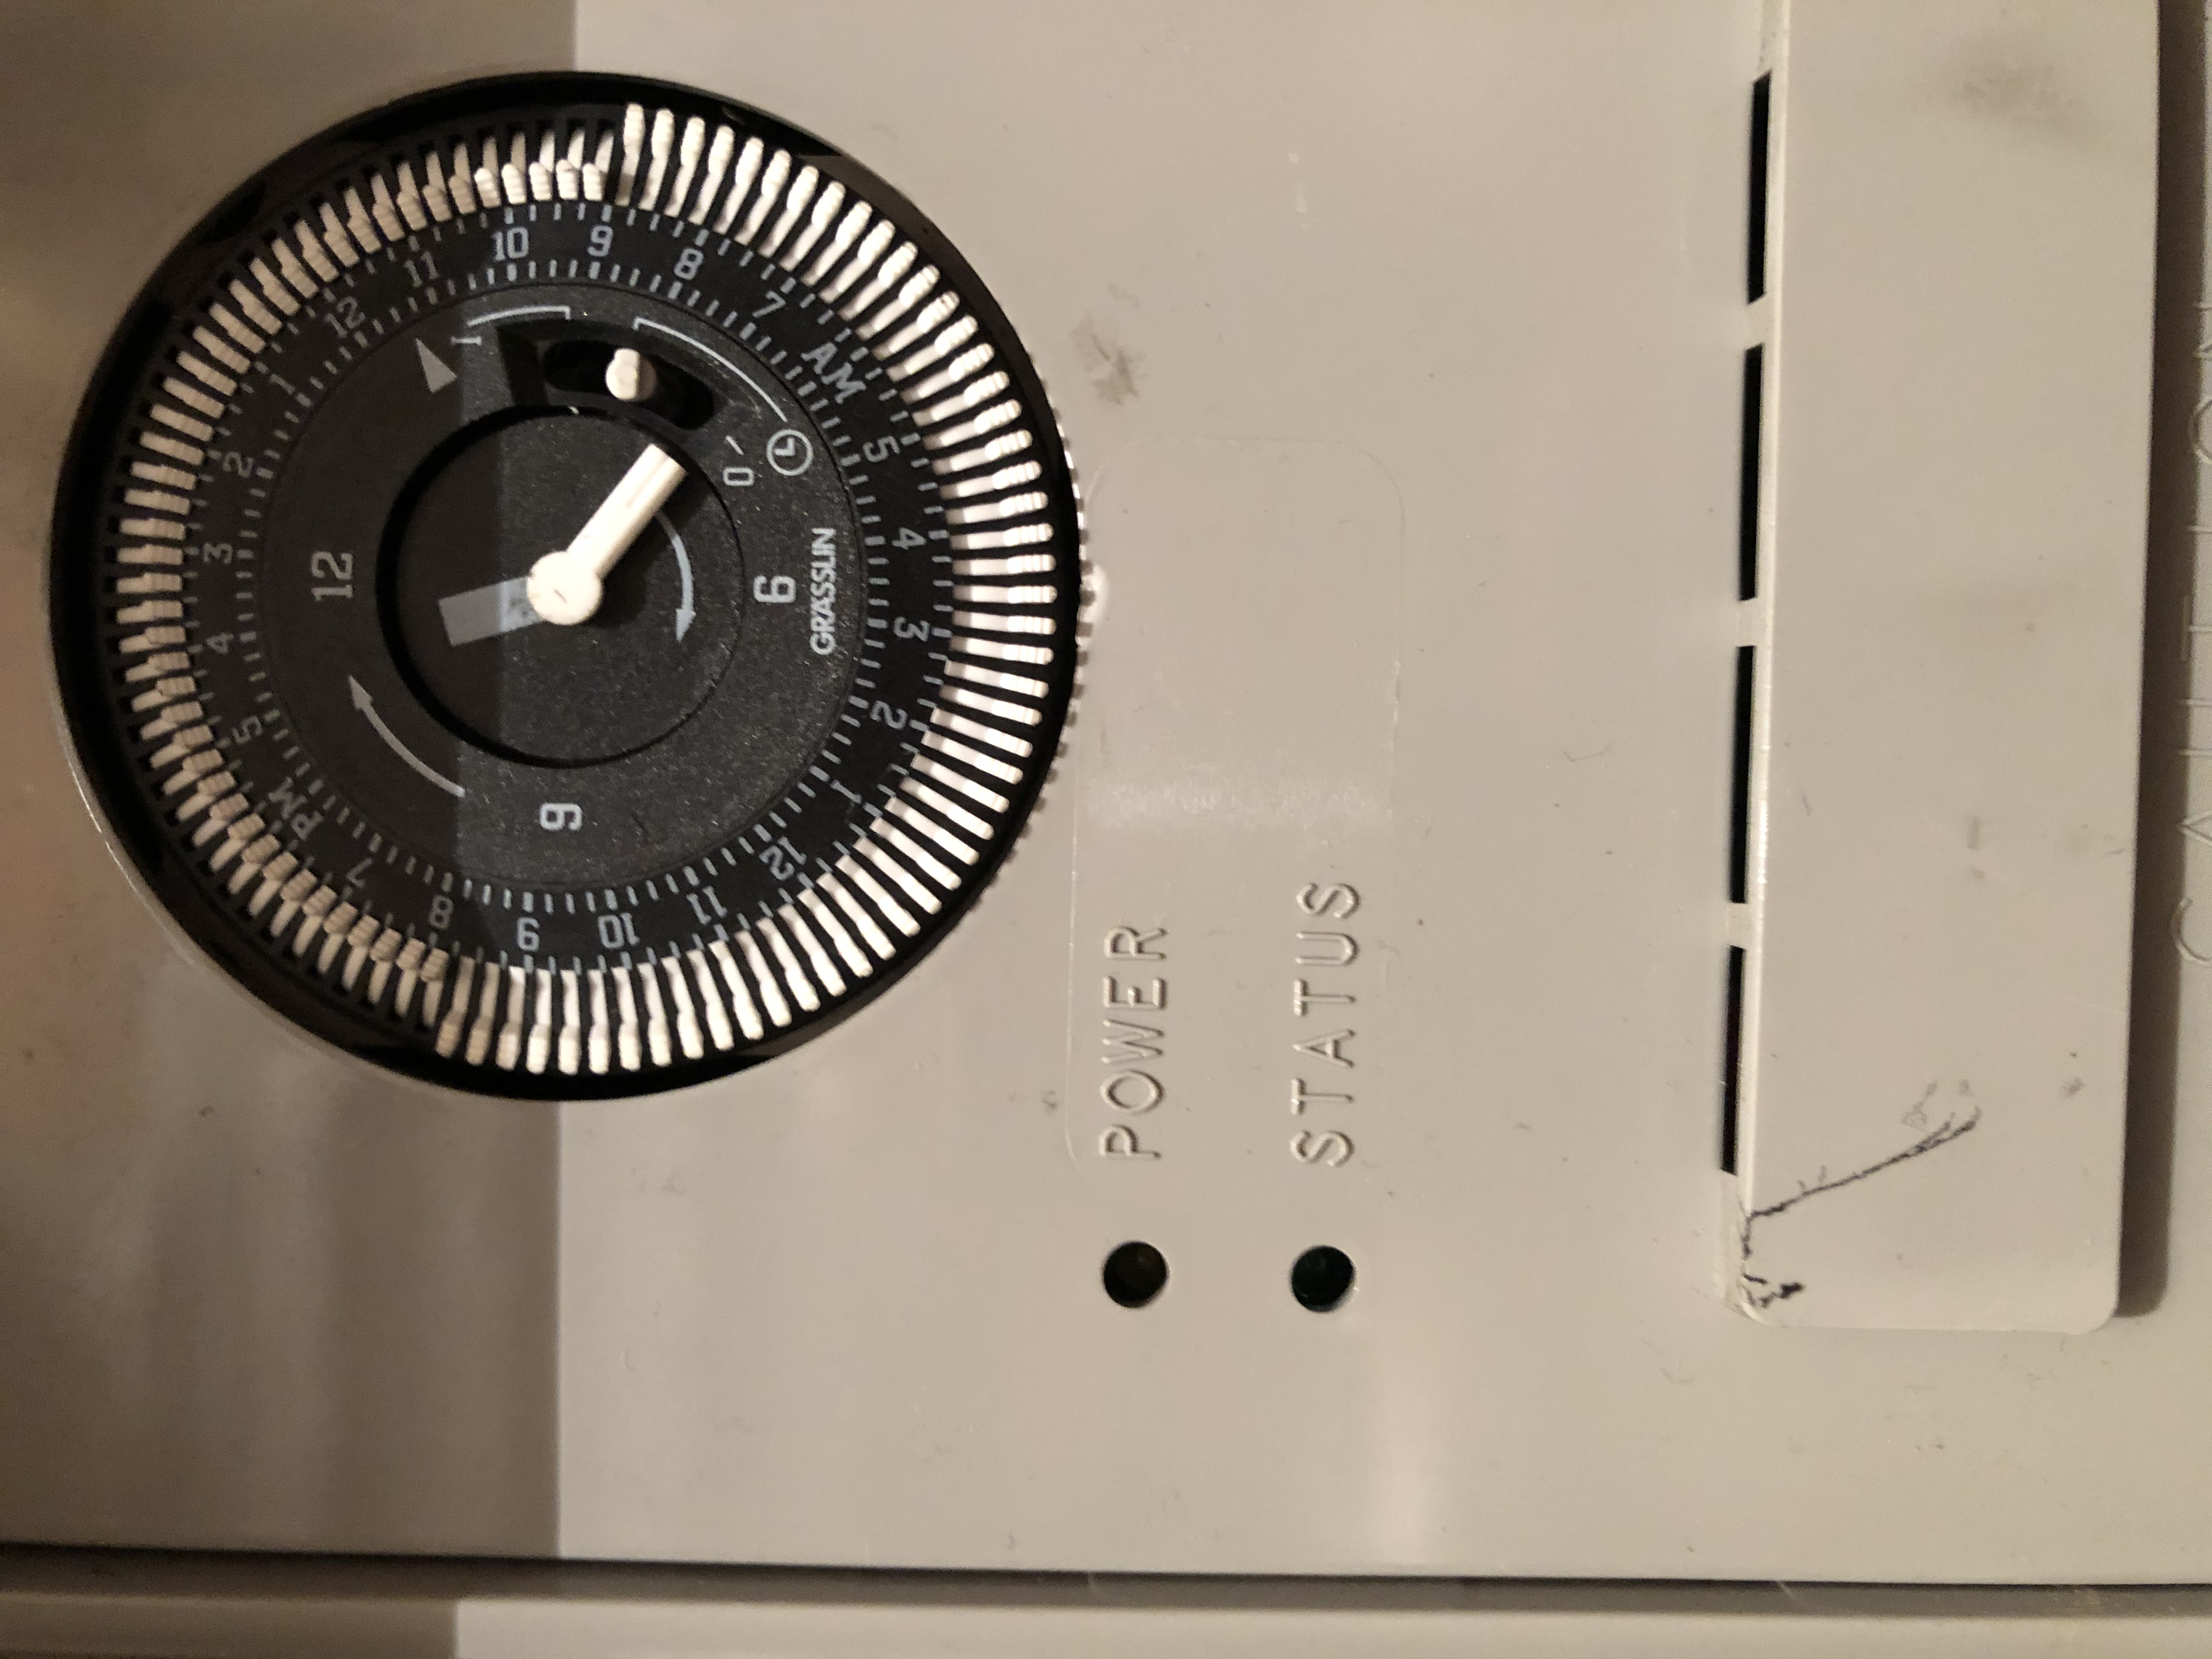
\includegraphics[width=\linewidth,angle=-90,origin=c,height=3.5in]{images/power-status.jpg}
  \caption{Power and status lights are off.}
  \label{Figure 1}
\end{figure}

\begin{figure}
  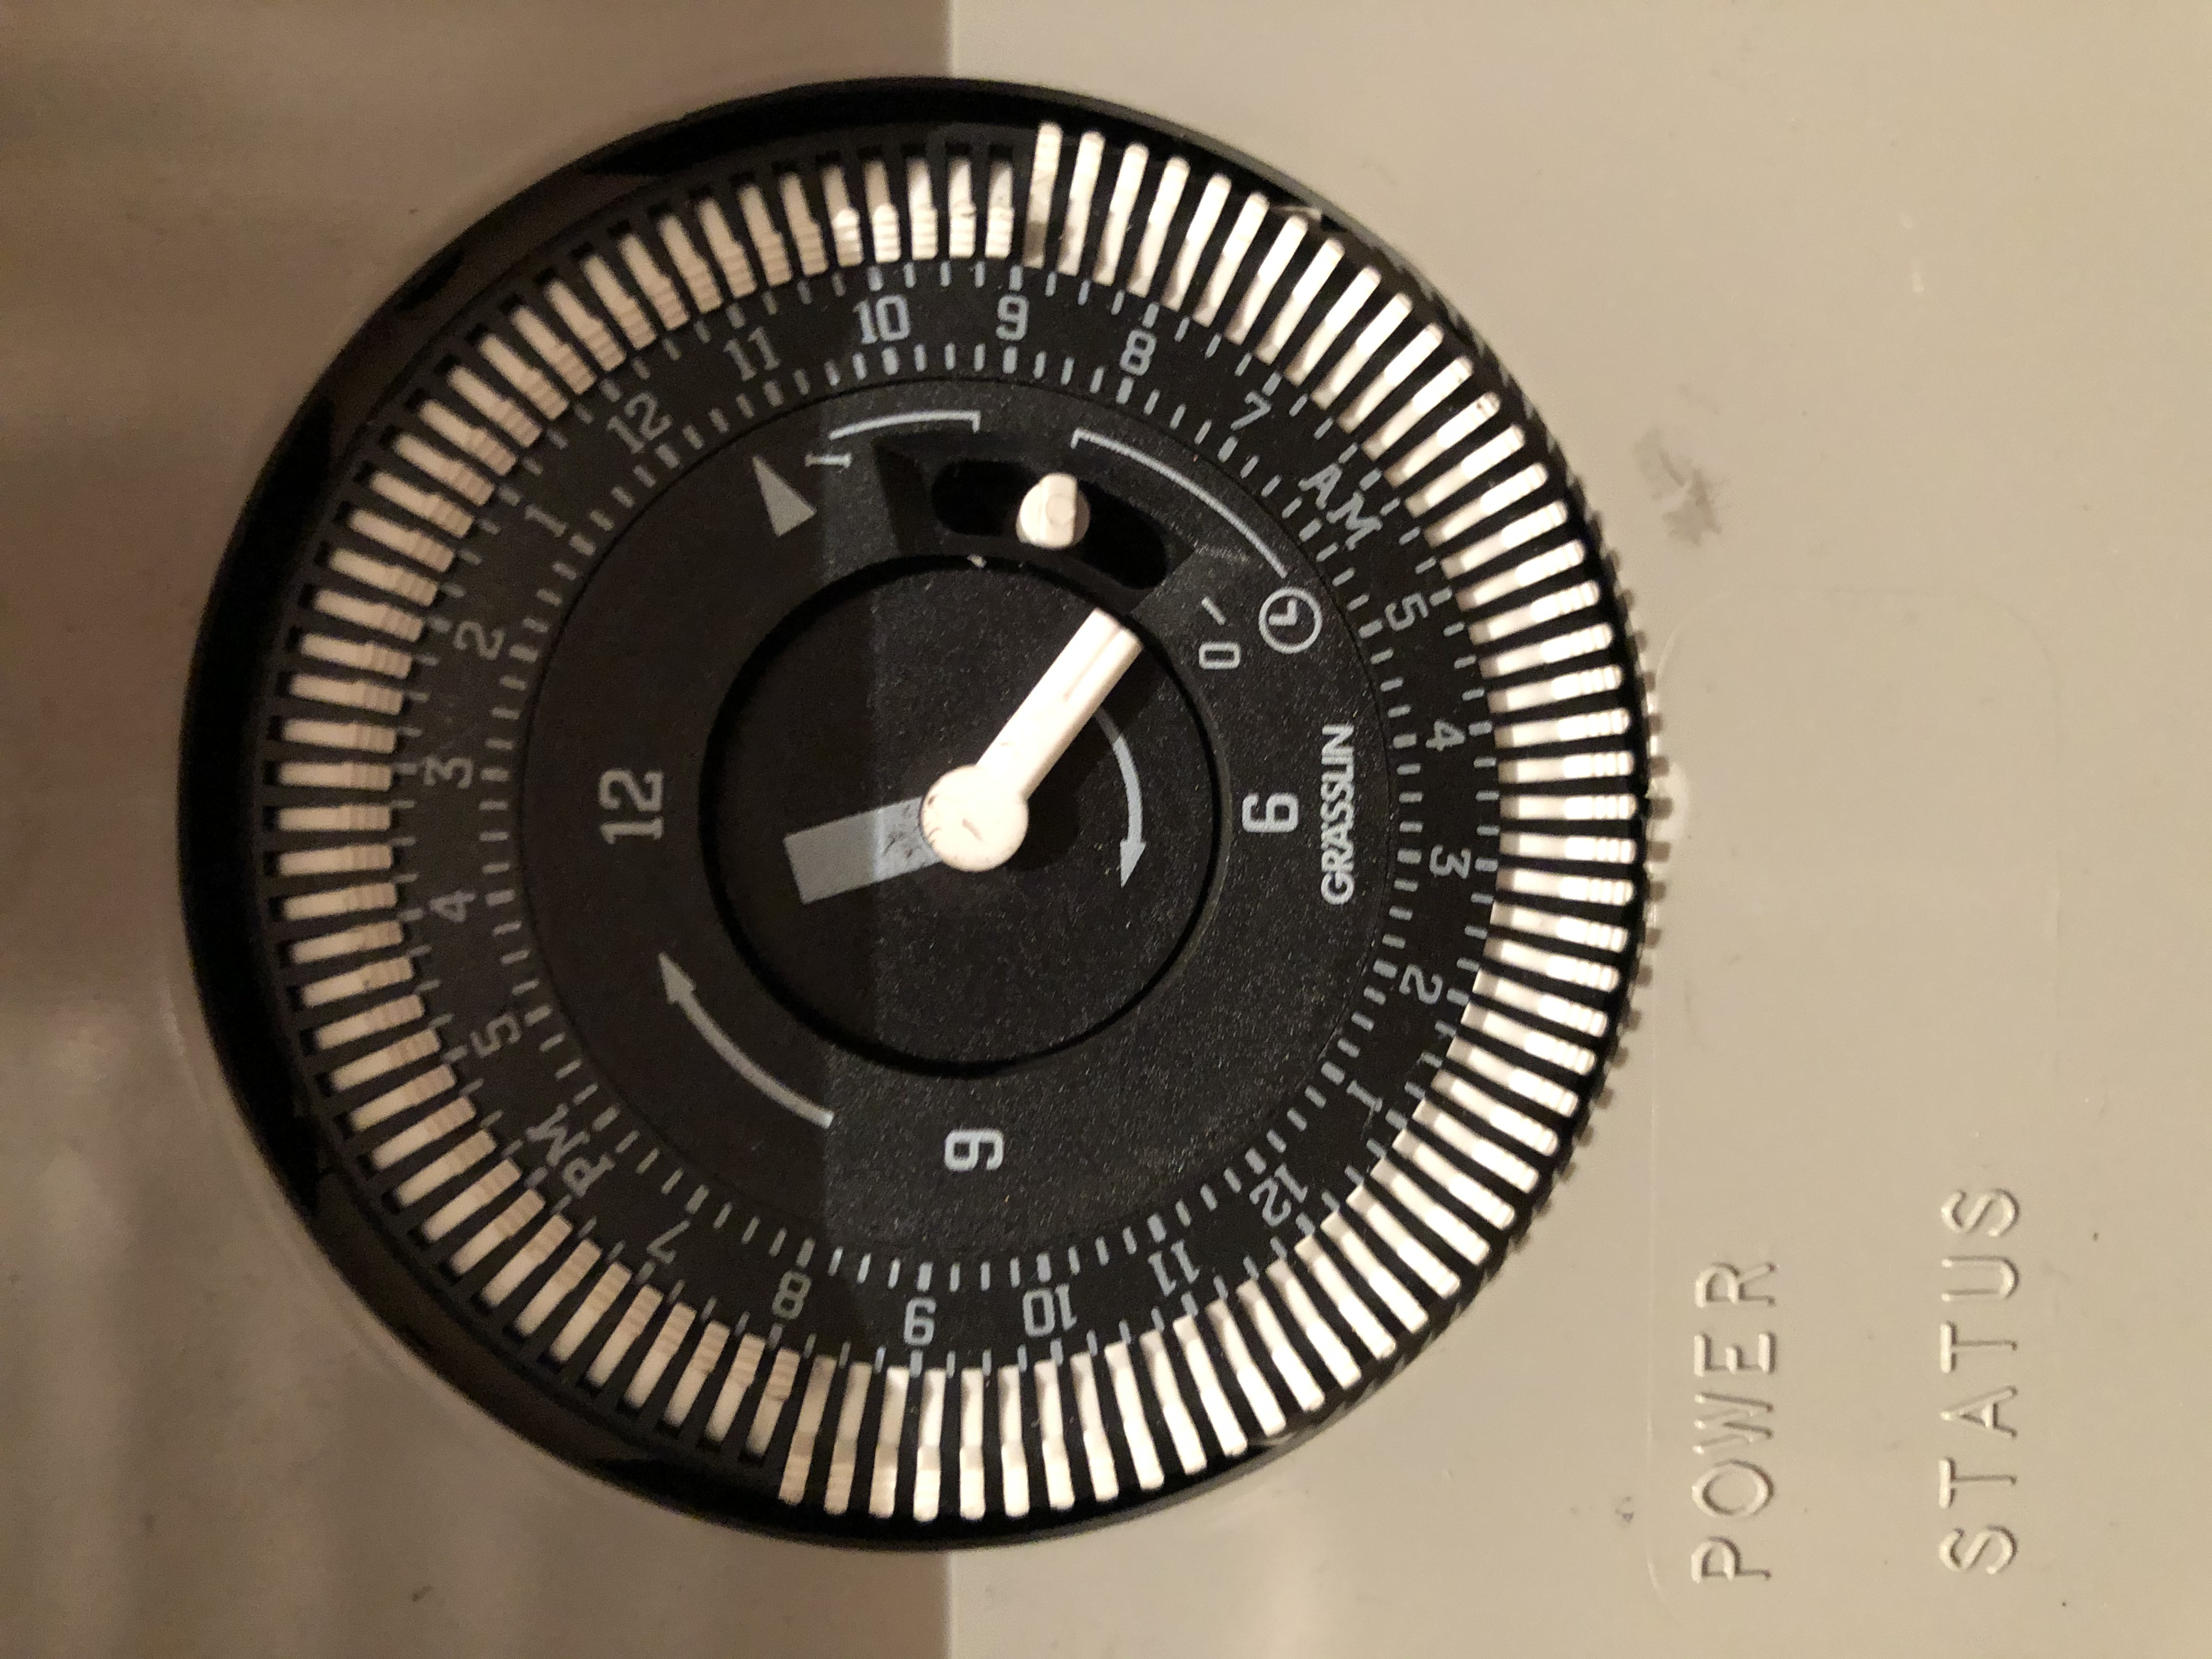
\includegraphics[width=\linewidth,angle=-90,origin=c,height=3.5in]{images/20200726T1014.jpg}
  \caption{Timer at 10:14 a.m. on July 26, 2020.}
  \label{Figure 2}
\end{figure}

\begin{figure}
  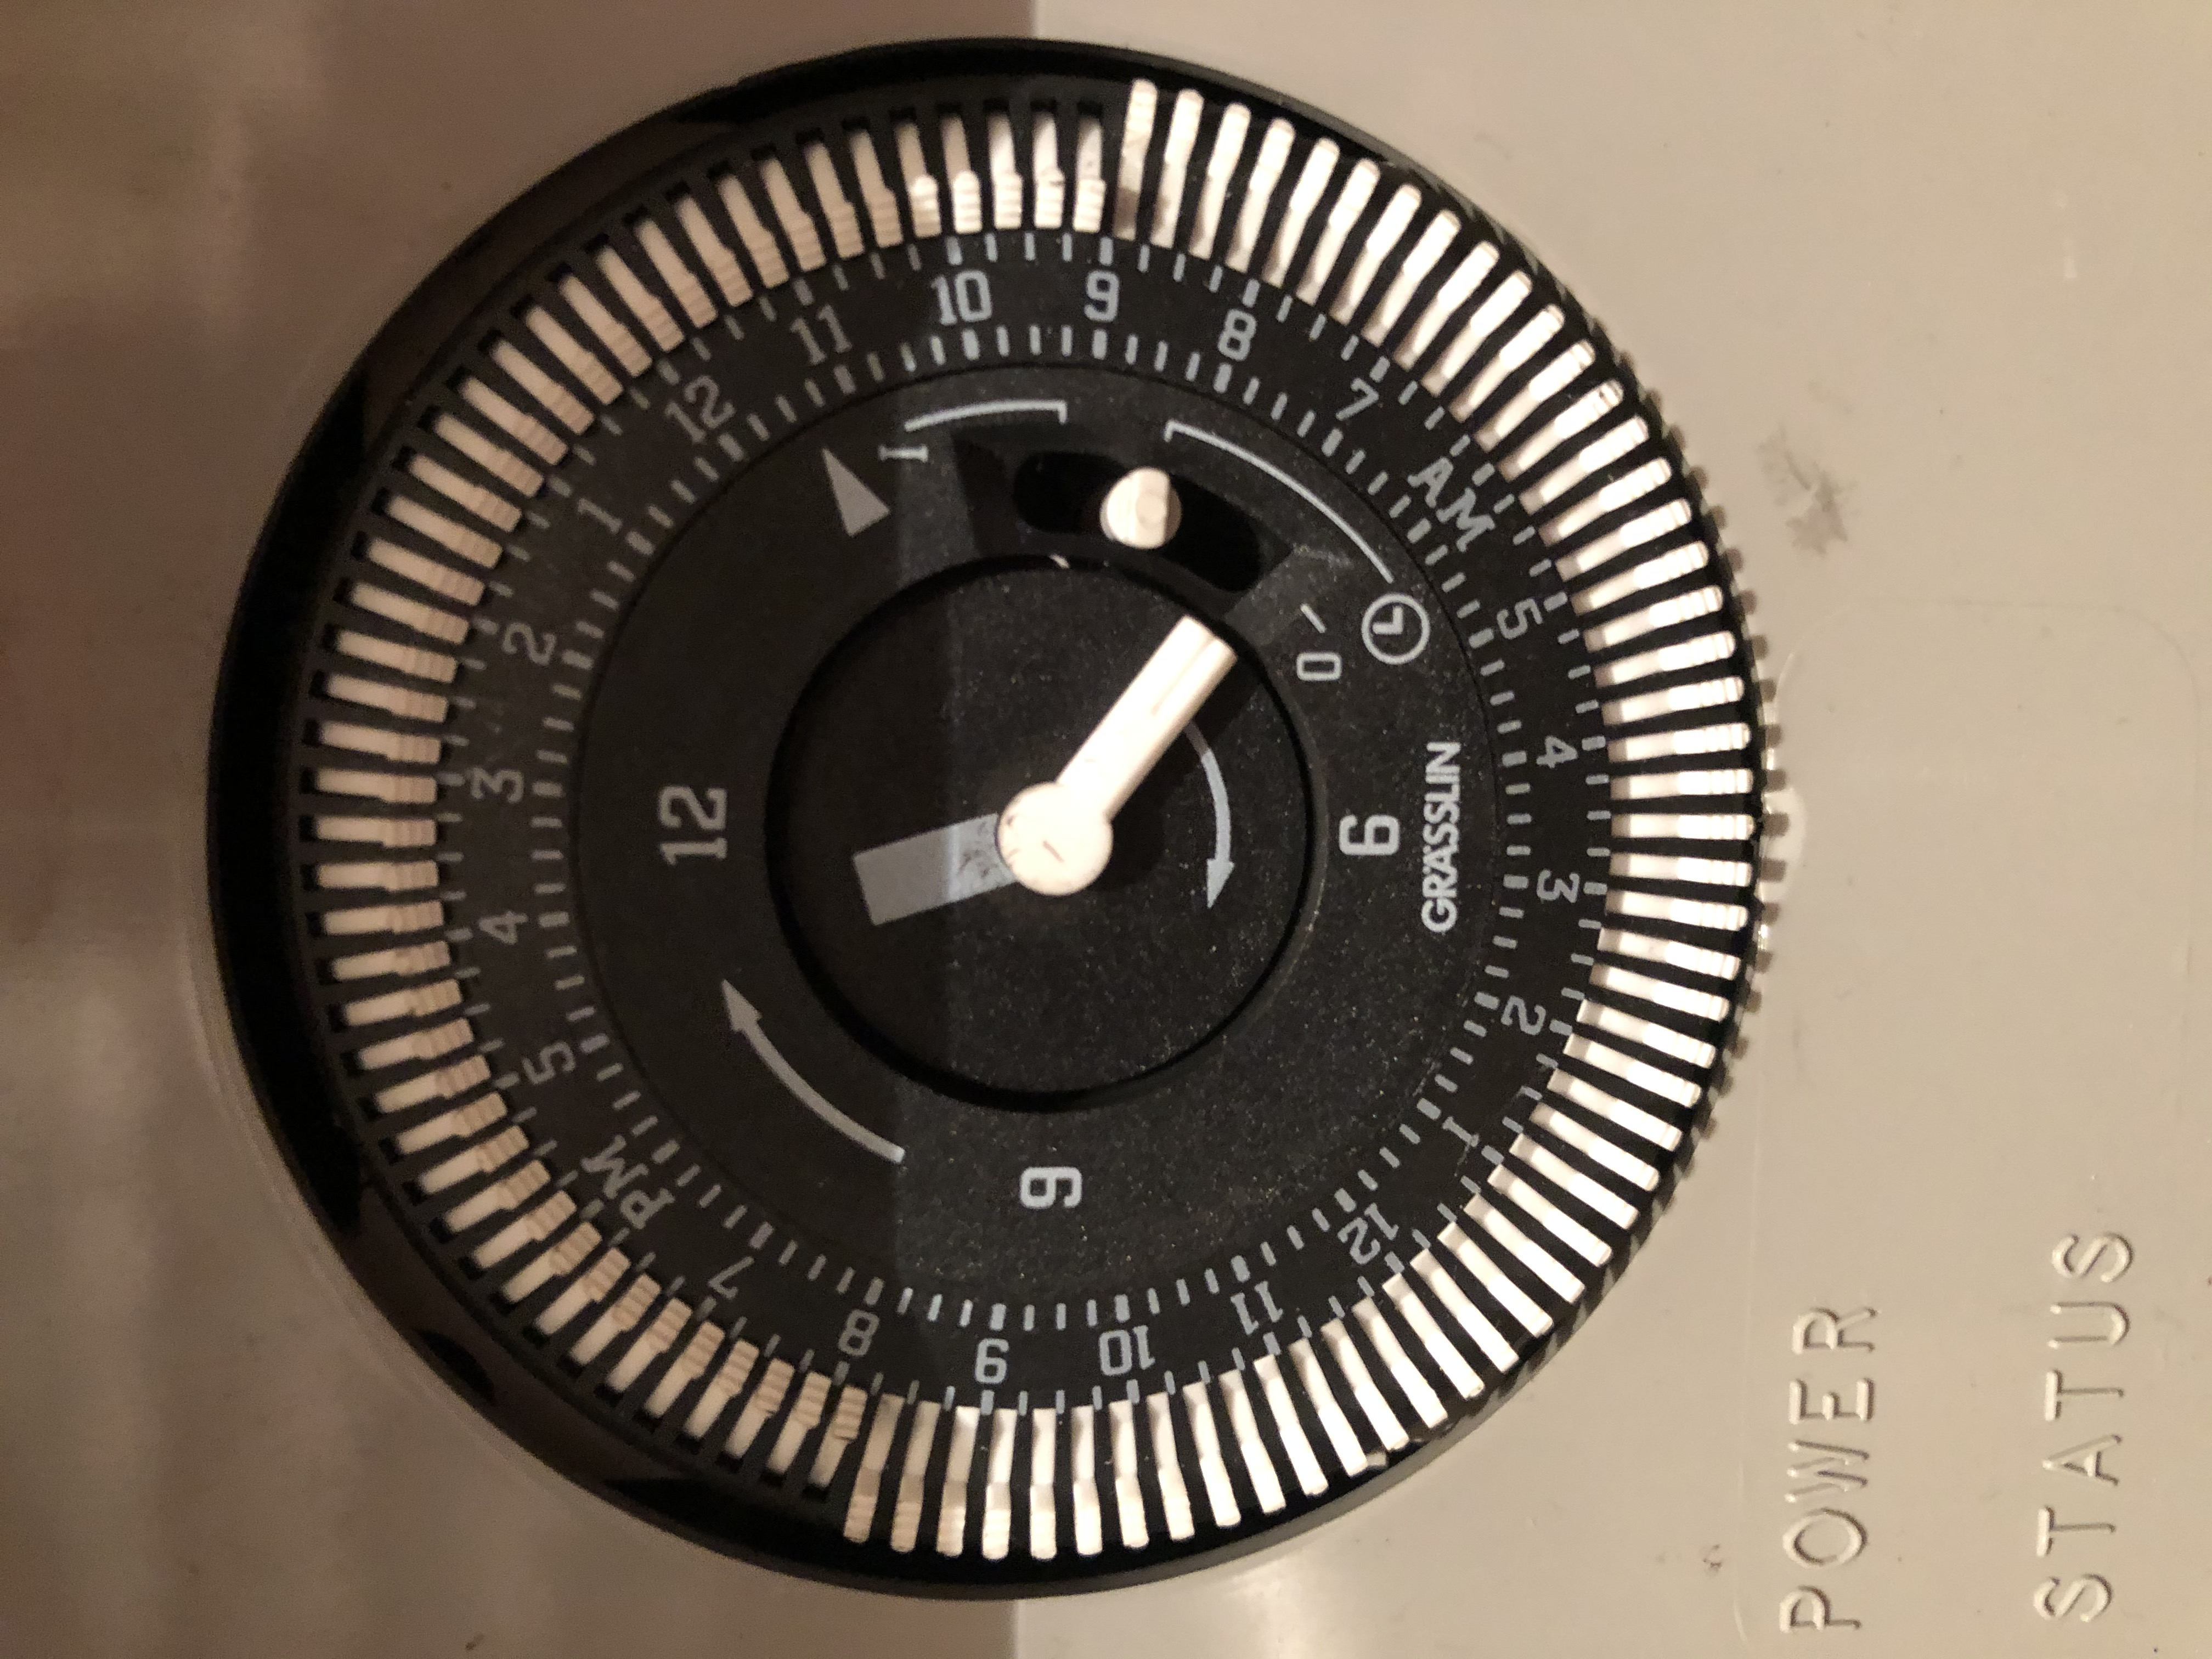
\includegraphics[width=\linewidth,angle=-90,origin=c,height=3.5in]{images/20200726T1440.jpg}
  \caption{Timer at 2:40 p.m. on July 26, 2020. Note no movement since 10:14 a.m.}
  \label{Figure 3}
\end{figure}

\begin{figure}
  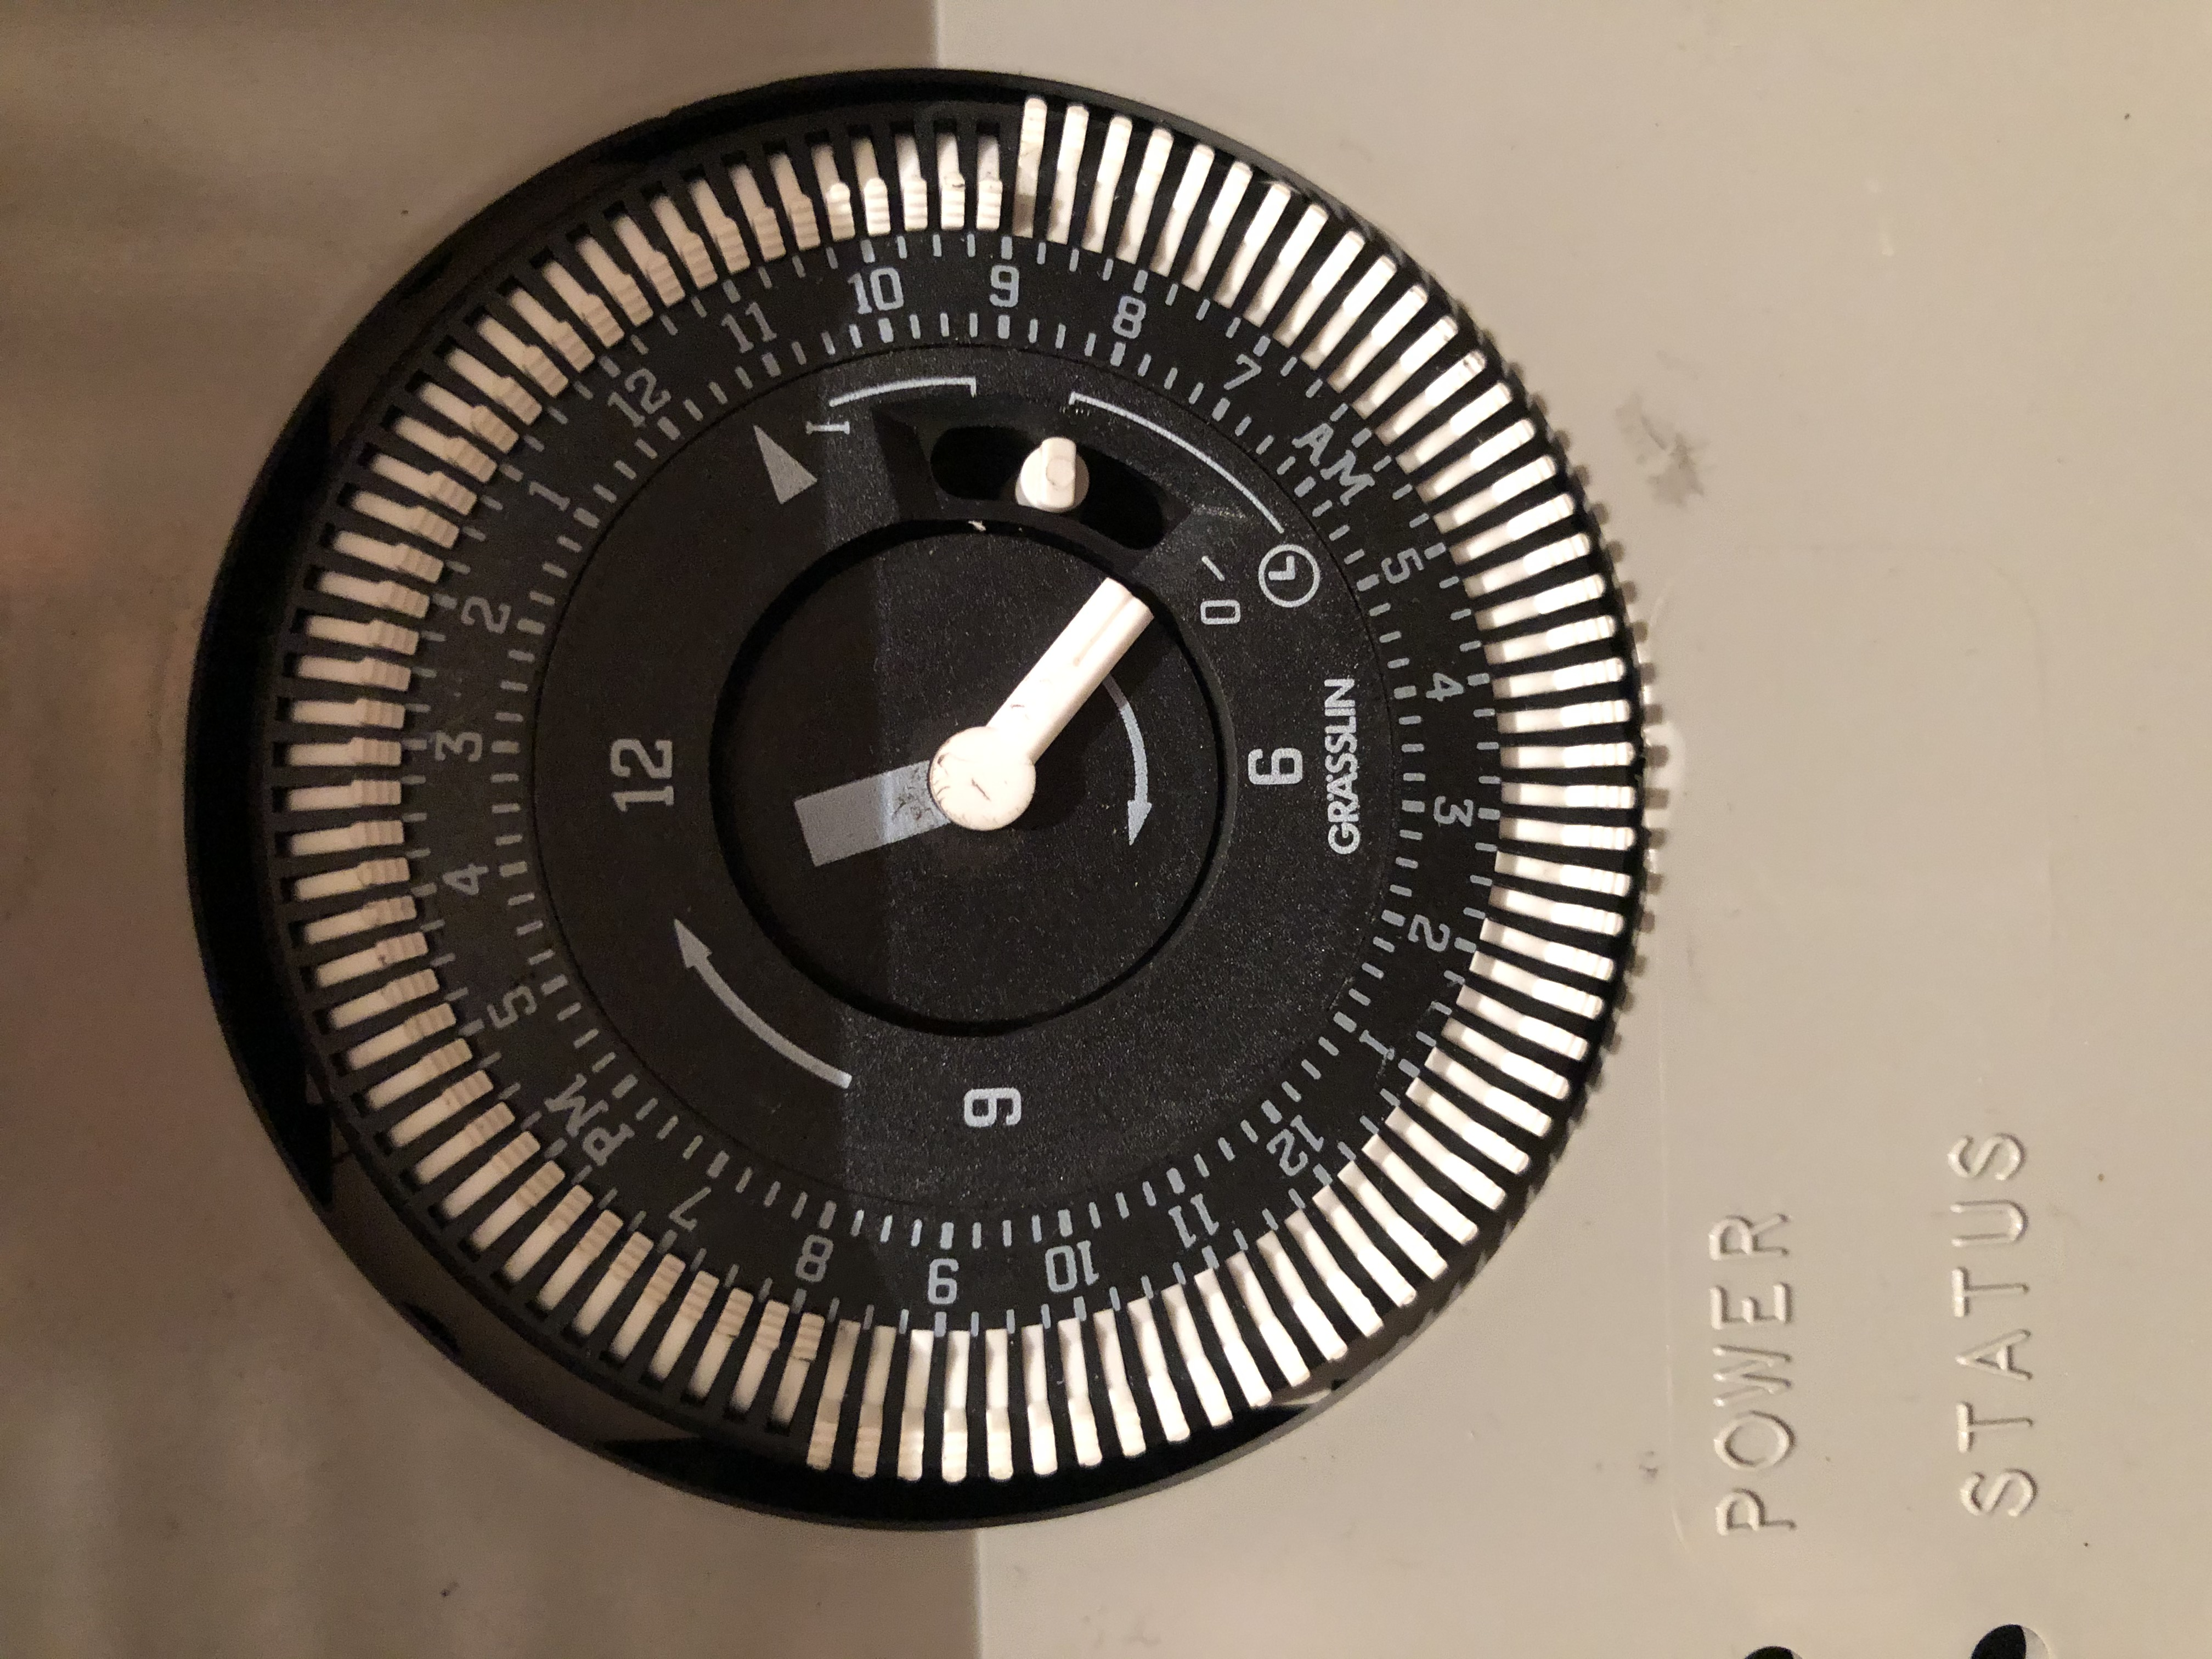
\includegraphics[width=\linewidth,angle=-90,origin=c,height=3.5in]{images/20200726T1720.jpg}
  \caption{Timer at 5:20 p.m. on July 26, 2020. Still no movement since 10:14 a.m.}
  \label{Figure 4}
\end{figure}

\begin{figure}
  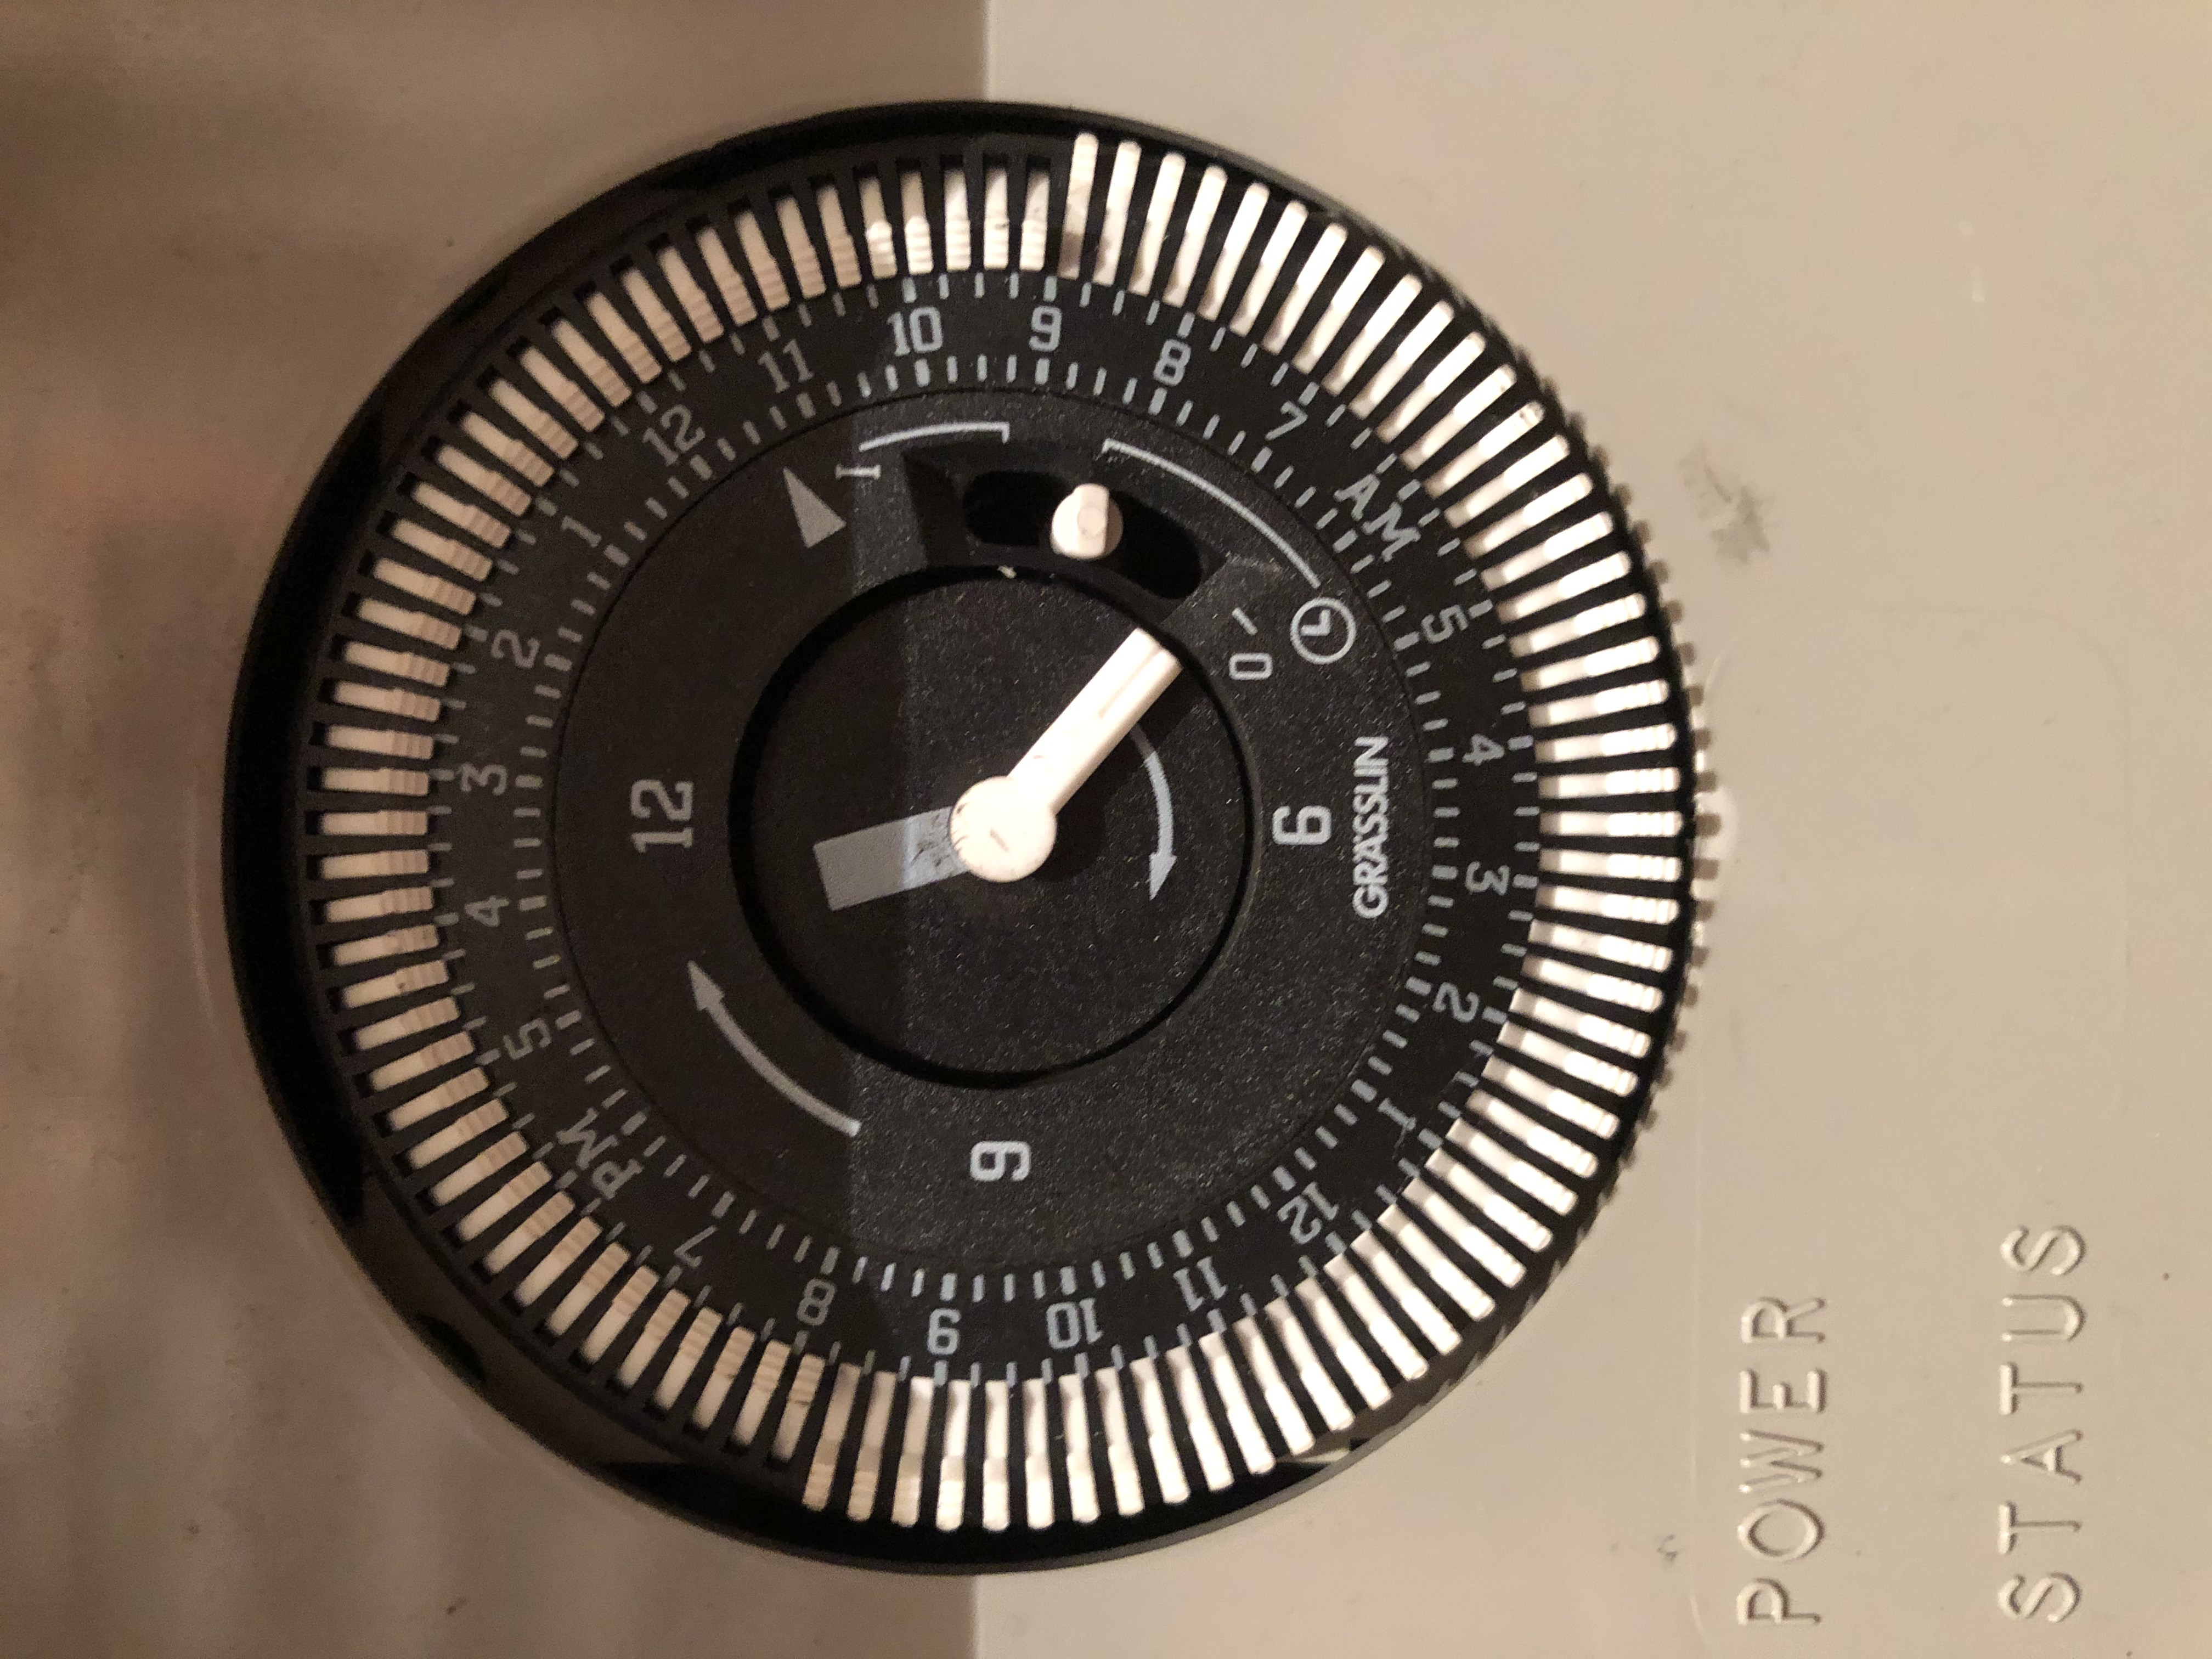
\includegraphics[width=\linewidth,angle=-90,origin=c,height=3.5in]{images/20200726T2122.jpg}
  \caption{Timer at 9:20 p.m. on July 26, 2020. Still no movement since 10:14 a.m.}
  \label{Figure 5}
\end{figure}

\end{document}
